%!TEX root = ../dissertation.tex

\begin{savequote}[0.6\textwidth]
	\itshape I suppose it is tempting, \\
	\itshape if the only tool you have is a hammer, \\
	\itshape to treat everything as if it were a nail.
	\qauthor{---Peter H. Salus}
\end{savequote}

\chapter{Introduction}
\label{chap:01}

\Lettrine{Since} their inception, computers have been intimately connected to all areas of engineering and science. In fields like molecular biology and chemistry, they can assist in problems such as optimization of chemical reactions, drug discovery, material design, or structural characterization. The term \textit{molecular modeling}, defined as the use of computational methods to describe the behavior of matter at the atomistic or molecular level,\cite{maginn2009} encompasses all these applications as part of a vast family of techniques and tools.

The increasing presence in molecular sciences (see \autoref[appendix]{chap:appendix-a}) must be also attributed to the efforts that the modeling community have been putting on two main fronts: user-friendliness and multiscale applicability. The former is devoted to creating intuitive interfaces with smooth learning curves, so that users can easily set up and analyze their calculations. This allows modelers to be more efficient and brings non-computational scientists closer to the field. The latter is concerned with joining distinct methods in a single coherent protocol to reach higher accuracy across different molecular scales. With this kind of protocols, phenomena ranging from recognition processes to catalysis can be accurately simulated. The success of these approaches finally crystalized in the 2013 Nobel Prize, granted to Warshel, Levitt and Karplus.\cite{nobel2013}

Building software that satisfies both requirements ---user-friendliness and multiscale applicability---, is not easy and requires an architecture that guarantees long-term development. A popular strategy consists of writing a robust core platform with a programmatic interface that supports the rest of features in the form of plugins or extensions. The core logic is usually written in a compiled language like C++, which provides high performance but slower development times. Once the heavy lifting is off-loaded to the core, the extensions can be written in more agile languages, like Python, Tcl or Ruby.

Among all the possible choices, Python has been the most successful over the last years, growing faster than any other language.\cite{stackoverflowpythongrowth} It has been chosen as one of the main development language in very popular companies and software products,\cite{pythonsuccess,googlepython,facebookpython,netflixpython} and, for the interest of this project, molecular sciences. Specifically, it can be found as part of PyMol,\cite{delano2002pymol} UCSF Chimera,\cite{chimera} OpenMM,\cite{openmm} Amber,\cite{amber} or Vina,\cite{trott2010autodock} to name a few.

Choosing Python is not a temporary trend, but a fully educated decision. It allows to abstract away technical details like memory management, so the developer can focus on the features of the project. Its high-level description and object-oriented architecture provides an intuitive mindset to create packages with a strong modular component. This makes Python the perfect companion for developing new molecular modeling strategies. For example, each method can be abstracted in a separate module, allowing to build multiscale protocols by simply chaining the interfaced functions.

The premises of this Ph.D. stand precisely on these aspects, mainly focusing on: (1) developing and applying a novel multiscale platform based on Python flexibility, and (2) generating a new paradigm in 3D sketching for complex molecular design.

This introductory chapter will provide a brief overview on: (1) the major software categories in molecular modeling, which will be further detailed in \autoref{chap:02}; (2) how they can be used together in integrative approaches; and (3) the difficulties, caveats and pending challenges present in these approaches.

\section{Molecular modeling: accuracy vs sampling}
% \addcontentsline{toc}{section}{In silico molecular modeling}

To understand the benefits of multiscale modeling, and why we need it, we must first review the available molecular modeling techniques: how they are used separately, and how we can join them together in a single protocol.

The most popular task performed in molecular modeling consists of describing the energetics of a system, which can then be used as a proxy for structure optimization, reaction path guessing or studies on dynamic behavior, among others. Depending on the method employed to obtain those energies, the results will resemble the experimental observations with higher or lower accuracy. In general, the higher the accuracy, the narrower the accessible search space (be it conformational or chemobiological, see fig. \ref{fig:multiscalethong}).

\begin{figure}
		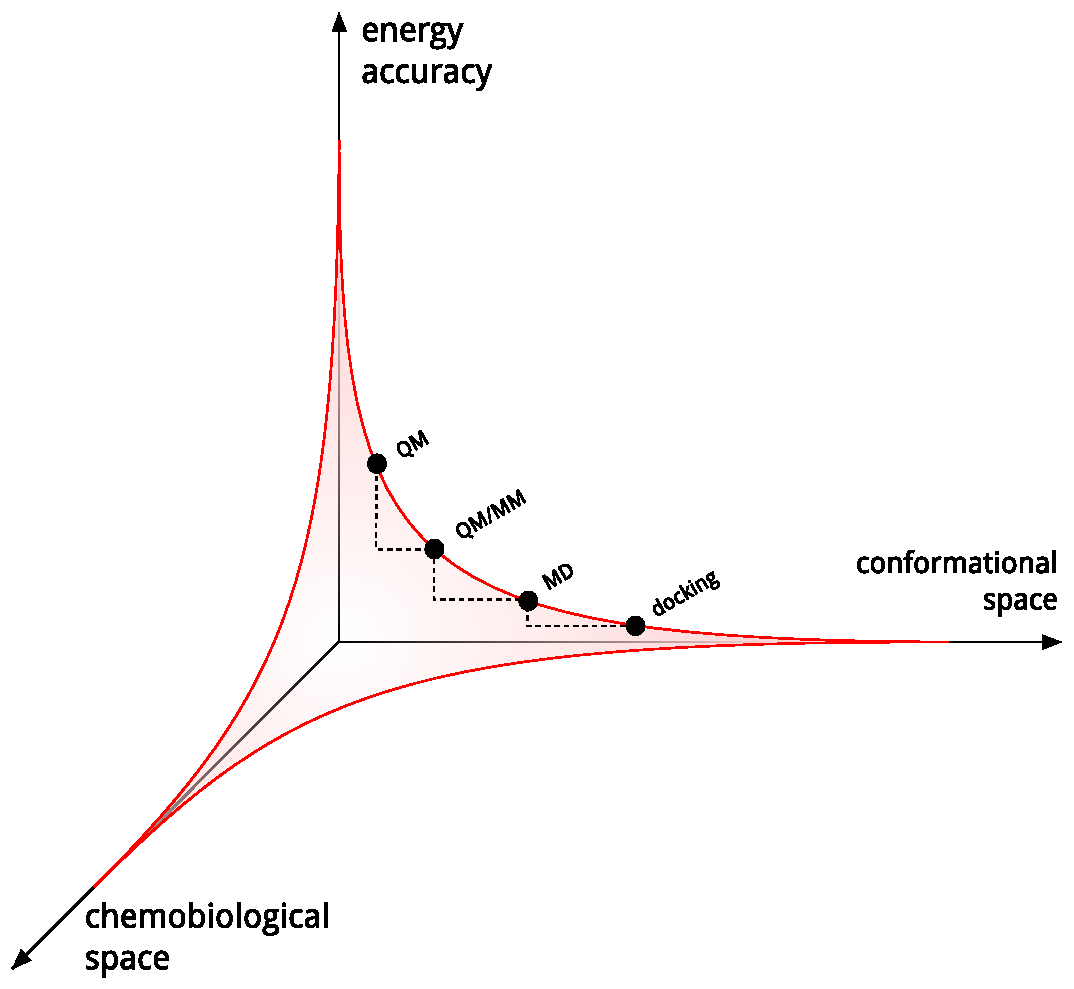
\includegraphics[width=\textwidth]{./figures/01/thong.pdf}
		\cprotect\caption[Accuracy vs accessible space in multiscale modeling]{When considering a multiscale protocol, one must face the compromise between the phenomena to observe and the reported accuracy on the results. Due to the limited availability of computational resources, one must face the compromise between large sampling capacities and accurate energies. Here depicted, a multiscale protocol on the conformational space.}
		\label{fig:multiscalethong}
\end{figure}


Atop the accuracy curve we can find Quantum Mechanics (QM) methods, which are based on quantum chemistry and the equations proposed by Schrödinger in 1925. This family of methods consider electrons explicitly, which allows them to study chemical reactivity with the highest precision. However, given the complexity of the calculations involved, even modern hardware cannot deal with more than a few hundred atoms, resulting in limited sampling capacity.

The next major family, Molecular Mechanics (MM), discards explicit electronics for the sake of speed and scale. Instead of applying Schrödinger's theory, it considers molecules as a set of spheres connected by carefully calibrated springs, whose energy is given by Newton's laws of motion. This results in much simpler calculations which can deal with thousands of atoms almost instantaneously. In fact, their most popular usage is its time-dependent implementation, Molecular Dynamics (MD), which analyzes the evolution of a system over millions of timesteps to obtain an accurate representation on the molecular behavior along a few nanoseconds.

QM and MM can be used simultaneously in the same system using an approach called QM/MM. This hybrid method allows to consider larger structures by splitting the calculations in two regions modeled differently. QM is applied to a reduced part of the system that requires an accurate electronic representation, while the rest of the structure is processed with the simpler MM techniques. Both calculations are then integrated by using hybrid schemes such as IMOMM,\cite{maseras1995imomm} IMOMO\cite{humbel1996imomo} or, most popularly, ONIOM.\cite{svensson1996oniom}

Even though it can be argued that energy calculations are behind every molecular modeling study, not all methods focus on obtaining an accurate value. Sometimes, a distantly close one is enough. For example, protein-ligand docking studies are designed to obtain probable orientations in which a small molecule (ligand) can bind to a bigger one (protein). For this assessment, obtaining an accurate binding energy is not as important as navigating the search space reliably: it is preferred to focus on the fast generation of reasonable candidate poses instead of a locating a true global minimum. To do that in an affordable time, accurate energies are normally replaced by scoring functions that return pseudo-energies or even unitless scalars. These functions can be based on simplified molecular mechanics, knowledge-based potentials, shape complementarity or even simple geometric measurements.

Drastic simplifications of energy are not uncommon in molecular modeling, especially if large search spaces must be analyzed efficiently. Normal Mode Analysis (NMA) apply an even simpler ball-and-springs model to obtain the principal vibration frequencies of a molecular structure. Under this approach, collective motions can be assessed in minutes without resorting to long molecular dynamics, which can take days or weeks to finish.

% Vast search spaces are not limited to macromolecules with large number of atoms. Every variable considered during an analysis generates an additional dimension in the search space. Any slight change in the topology of the molecule can incur in more complexity, such as exploring point mutations in the protein sequence (biological space) or testing different functional groups in one part of the ligand (chemical space). Exploring (bio)chemical spaces require very specific tools and there is no general-purpose utility in that regard. For chemical spaces, QSAR (for Quantitative Structure-Activity Relationship) can be applied: these are classification or regression methods that can predict chemical properties of a compound (like biological activity of a drug) by relating key properties in big datasets (presence of certain functional groups, for example).


\section{Multiscale and integrative modeling}
% \addcontentsline{toc}{subsection}{Multiscale and integrative modeling}
%

Few computational studies are composed of only one step that relies on a single program to obtain a one-shot result after the first calculation. They usually comprise multiple stages that combine several theory levels and software packages to achieve the intended results. This is especially true in multiscale approaches, as pointed out by Grimme and Warshel (see \autoref[Appendix]{chap:appendix-a}).

Multiscale modeling is often necessary because many molecular phenomena comprise a wide range of magnitudes at different scales. For example, studying the entire mechanism of an enzymatic reaction would require the description of binding processes and catalytic mechanisms, leading to the need of both a wide conformational sampling (docking, large scale or steered MD) and fine electronic treatment (QM or QM/MM), respectively.

The consequences of having different methods for varying sizes and timescales is that those methods must be combined in well-designed hybrid protocols. There is no clear strategy that dictates the proper sequence of methods and levels of theory. Most common strategies start with less accurate methods like docking, select some poses for further assessment using MD simulations, and pick some representative states to be optimized in QM or QM/MM schemes \todo{Citation needed} (see fig. \ref{fig:multiscale}). However, depending on the information available, a study can begin with a DFT optimization of a reduced model and then progressively consider more atoms by decreasing the method accuracy: freezing some atoms in a cluster model, using semi-empirical approaches or hybrid methods and finally checking stability with a MD simulation \todo{Citation needed}.


\begin{figure}[H]
		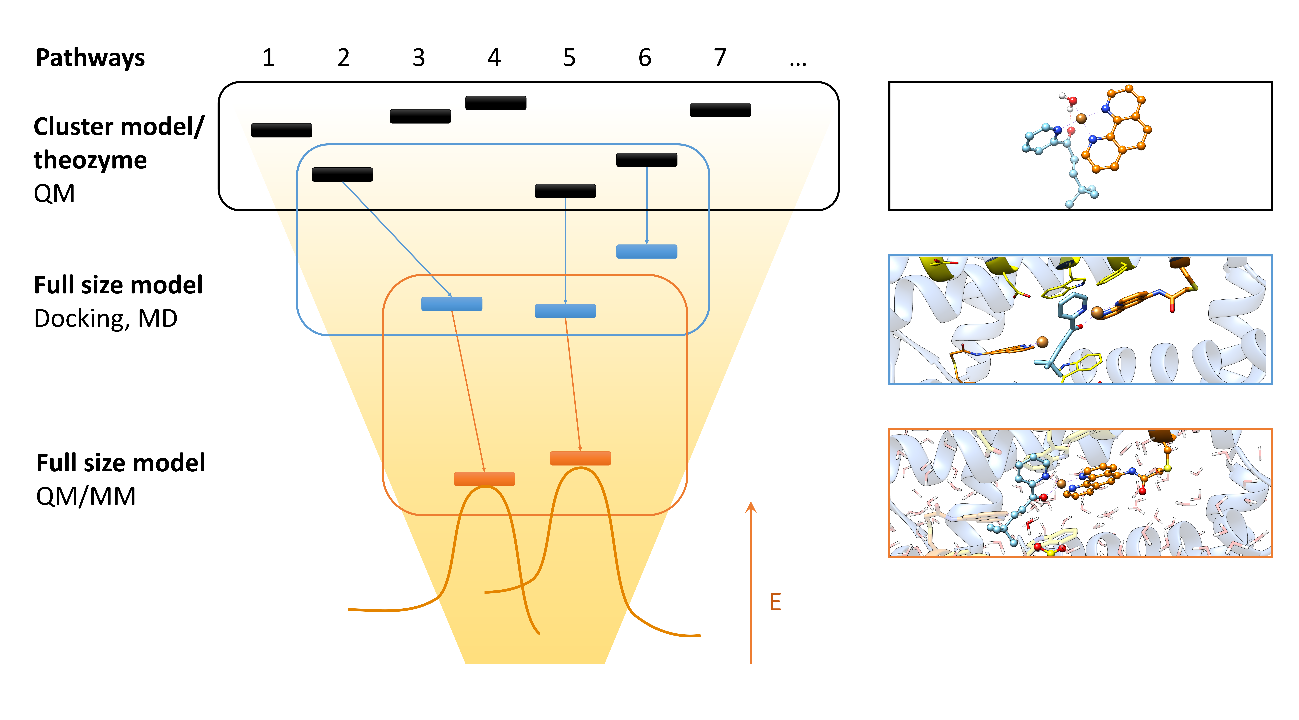
\includegraphics[width=\textwidth]{./figures/01/multiscaleprotocol.png}
		\cprotect\caption[Example of a multiscale protocol]{Example of a multiscale protocol applied for the identification of the catalytic mechanism of a metallic cofactor inside a metalloenzyme. (Reproduced from \textit{Computational Methods in Enzyme Catalysis}).\cite{EnzymeDesign2015}}
		\label{fig:multiscale}
\end{figure}

Every study is different and presents unique scientific and technical challenges, which are almost always overcome on an individual basis. Workarounds, patches and scripts are so commonly needed that it becomes an art on its own. In the future, this will be less of an issue as hardware gets faster and software smarter, but in the meantime standardizing some common workarounds can produce successful results. For this to happen, one must first understand those challenges.

\subsection{Dealing with software fragmentation}
% \addcontentsline{toc}{subsection}{Dealing with the software fragmentation in molecular modeling}

The vast landscape of molecular modeling comprises hundreds of programs that have been developed to address different problems and, most of the time, with only that problem in mind. They were not designed to be part of a bigger, integrated workflow. Subsequently, good integration is needed between the involved software, which, unfortunately, it is not always the case.

Each of the steps will require different information depending on the supporting theory (in addition to atoms and coordinates, some will need connectivity, residue grouping, charges, parameters) and each of the involved programs might exhibit slight differences in how the exchanged files are parsed or exported. For example, one particular tool handles element names as case-independent, while the next one would only accept uppercased names. One tool might use different unit systems and a conversion is required (nanometers and angstroms is a common one). As a result, even after managing to correctly thread the needed file formats as required, a robust behavior of the workflow is not guaranteed and ends up in fragile, unexpected performance.

This is both cause and consequence to the absence of a standard file format to deal with biomolecules and chemical compounds. On the contrary, first projects created custom file formats to deal with their own necessities, which has led to several file formats coexisting with an overlapping feature set. \texttt{XYZ} is the simplest, with only providing a list of elements and their coordinates, line by line; crystallographers use \texttt{PDB} files to handle big macromolecular structures such as proteins; MDL (now part of Dassault Systems) created \texttt{MOL} and \texttt{SDF} files to deal with small compounds; Tripos’ Sybyl (now part of Certara) introduced \texttt{MOL2} for their docking studies\ldots  only to name a few.

After many years of battling the file format war, a true standard is yet to be defined. While there are ongoing efforts trying to solve part of the issue (the crystallographic community is slowly replacing the troublesome PDB file format with mmCIF\cite{bourne1997,berman2007}), new developments still have to deal with multiple input and output files to be competitive (see fig. \ref{fig:xkcd}). Some projects exist to cover the compatibility issues, such as the popular OpenBabel suite, \cite{oboyle2011} but that constitutes only a band-aid and not a true solution.

\begin{figure}[H]
	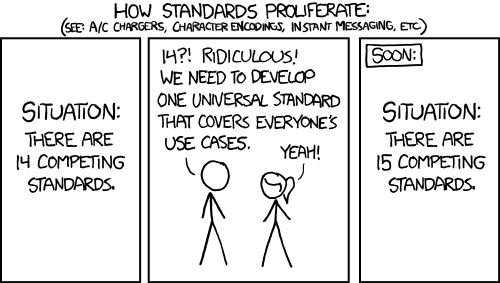
\includegraphics[width=\textwidth]{./figures/01/xkcd927.png}
	\caption[Proliferation of standards]{How standards proliferate. Reproduced from XKCD 927 (\url{http://www.xkcd.com}).}
	\label{fig:xkcd}
\end{figure}


The solution to this fragmentation is not an easy feat, and several strategies could be implemented to alleviate the issue. The first milestone is, simply put, write good documentation: time-tested protocols, which detail the software and versions used in each step are of utmost importance. If files need to be converted and/or edited along the process, these modifications must be noted too. Of course, this is only a patch and does not solve the background problem: format fragmentation. In this matter, several software-only attempts have been made and will be further detailed in the next section.

\subsection{The ecosystem of integrative platforms}
% \addcontentsline{toc}{section}{State of the art of integrative strategies}

Graphical user interfaces (GUIs) are designed to provide a common workspace in which all  operations can be carried out in a cohesive user experience. This avoids having to change contexts and learning new gestures for different tasks.

For molecular modeling, the perfect GUI would consist of a robust software platform that could act as the central hub for all molecular modeling programs, interfacing all of them seamlessly. In this sense, commercial graphical suites are likely the best option, since they have the means to build optimized interfaces for a broad range of computational workflows. Their main problem is, obviously, the licensing costs. Fortunately, alternatives exist for the academic users, be it special discounts for universities or free, open-source software developed by computational research groups. After all, a big part of the features present in commercial suites comes from academic developments (see \textit{charmm} vs \textit{CHARMM} vs \textit{CHARMm (Biovia)}, or \textit{AmberTools} vs \textit{Amber}).

\subsubsection{Commercial suites}
% \addcontentsline{toc}{subsection}{Big companies, huge market, large scale economics}
Molecular modeling companies build products to appeal all audiences, from novices to experts. While advanced and expert users have no problems in dealing with command line interfaces and text edition to manage programs, beginners usually tend to favor graphical interfaces. Dialogues, buttons and dropdown menus are way easier to handle than input files with arbitrary syntax. As a result, most commercial suites are graphical ones, creating the \textit{molecular design software} concept: a graphical interface that provides a real-time visualization of 3D structures with interactive building and conformational modification. On top of this interface several functionalities can be added, such as assembling polymeric, periodic or solvated systems, guessing partial charges, geometry optimization, force field parametrization and much more. Depending on the tasks the user is going to perform more often, some differences can be drawn, but overall the most popular suites will offer the same feature set.

As of 2018, a handful of suites can fulfil the aforementioned requirements: Schrodinger's Maestro,\cite{maestro} Dassault Systems’ Discovery Studio (formerly from Accelrys, now part of Dassault as Biovia),\cite{biovia2017discovery} Chemical Computing Group's Molecular Operating Environment (MOE)\cite{chemical2016molecular} or OpenEye Lead suite.\cite{openeyelead} Obtaining access to these suites is subject to a one-time or periodic license, which even with academic discounts, can sit up well in the thousands. Even with those prices, it seems to be worthy: the sector is growing year after year and the forecast for the next decade are very optimistic.\footnote{A study by Industry Arc Research projected that the Computational Medicine and Drug Discovery Software would reach 6.78 billion USD by 2020,\cite{industryarc} which agrees with GrandView Research studies: the structural biology and molecular modeling market will be worth 13.1 billion by 2025.\cite{grandviewresearch} According to a study published by Accuray Research in May, 2017,\cite{Accuray} which cites companies such as Accelrys, Certara, CCG or Schrodinger, the global computational biology market will reach a value of 11.25 billion USD by 2025. More studies on biosimulation, offer markets worth up to 2.88 billion by 2022.\cite{marketsandmarkets} This has been known for investors, of course, as evidenced by the 10 million USD round received by Schrodinger LLC from Bill Gates in 2010.}

Privative but free, SAMSON Connect (for Software for Adaptive modeling and Simulation Of Nanosystems) seems like a modern alternative backed by Inria. It requires an account and accepting their terms of use just to download the software, which includes a clause stating \textit{You must be at least 18 years old to use the Service}, restricting their use in the school. That said, it offers a good software development kit (SDK), backed by good documentation on how to write custom \textit{Elements}  or extensions which are distributed through their online community. However, after further inspection, one quickly realizes that they are primarily focusing on materials design and nanosystems, not macromolecules and small compounds.

% \missingfigure{Top 10 Pharmas with computational departments by job offerings} % FIXME!

\textit{All that glisters is not gold}, said Shakespeare. All-in-one solutions, as provided by commercial suites, are very appealing to novice users, but when the intended purposes of the tool must be pushed, the commodities of the graphical become an impediment instead. This is crucial when modeling new areas of structural biology or organometallics, such as artificial metalloenzymes or metal-organic frameworks. In these frontier-fields, researchers cannot simply rely on existing protocols and tools, they create their own by trial-and-error or even code new algorithms to overcome the difficulties. In other words, the state of the art is not always available within the licensed suite, whose update might come a year too late.

It is true that through extended configuration files, some hardcoded parameters can be modified and, if the software features a decent Application Programming Interface (API), scripting languages can be applied to implement new algorithms and techniques. Modifying the source code is normally not possible because, being commercial, the source is not disclosed. If they do release it as open source, it is for an old version that, while helpful, it is not ideal.\cite{delano2002pymol} In that matter, the academic and/or open source software have a clear advantage.

\subsubsection{Academic software}
% \addcontentsline{toc}{subsection}{The ecosystem of academic software}
While there are software companies that do some research and develop new methods, only a handful publish their results, so it is fair to assume that most of the public knowledge comes from publications submitted by academic research groups. After all, most of the commercial scientific software was, at some point, of academic nature.\cite{gaussian,schrodingerpymol}

The academic landscape is not only broad, but also disperse. Lots of small projects are released weekly and it is very difficult to keep track of them all. A couple of web directories have emerged recently,\cite{omictools,pirhadi2016open} giving a small insight into the field. In OMICTools, only the proteomics category displays almost 9000 entries. GitHub,\cite{github} the de-facto online repository for open-source software, shows more than 2000 repositories for \textit{chemistry} searches.

When it comes to integrative suites, the analysis is much simpler. Few groups can dedicate all their efforts to building a wide-spectrum tool, especially when the commercial suites are well-established. If any, the one weakness that can be easily exploited is price: releasing an open-source tool with a comparable feature set would be very competitive.

One the best attempts to fill the gap is the UCSF Chimera project. First released in 2000\cite{firstchimera} and published in 2004,\cite{chimera} after 18 years of development UCSF Chimera shows its age: the graphical interface looks dated and, with today's standards, clunky. But that age is also a blessing: the software is stable, robust and mature, and accumulates a lot of modules to perform all kinds of analysis: clashes detection, H-bond depiction, density map fitting, peptide building\ldots  It comprises a huge number of small tools that, together, make for a good modeling suite. However, the diverse origin of the tools (some are built by the Chimera developers, but a good part comes from third-party collaborators), end up creating a feeling of unstructured workflow. It also lacks key elements like Quantum Mechanics integration or a modern Molecular Dynamics program (it does include MMTK, an abandoned project that cannot provide the performance expected with modern architectures).

This is caused by three main issues: (1) There is no developer documentation. The few resources are scattered between the mailing list and the Python code itself. (2) 15 years of back-compatibility surely comes with a price, which means shipping old projects with deprecated dependencies. (3) A deliberate isolation of the platform to ensure consistent behavior in all platforms prevents the developer from writing software with modern tools and libraries. Solving point (1) would be a huge effort that only the developers could satisfy adequately, but points (2) and (3) can be addressed with patches and clever workarounds, which are the reasoning behind one of the developments presented in this thesis (see \autoref{chap:05}). Fortunately, the same team behind UCSF Chimera is now working on ChimeraX, focused on the migration to modern standards and providing a central repository for 3\textsuperscript{rd} party extensions (the \textit{Toolshed}). While the core code is now available (and with proper documentation), the extra modules would take more time. This means that the feature set is yet to be comparable.

Classic visualizing software like VMD or PyMol could also fill the gap: they have been developed for years and now accumulate a good number of extra features thanks to the contributed extensions. The problem is that they lack an attractive, intuitive interface to begin with and both feel like a modest 3D viewer with extra modules bolted on: functional, but not ideal. The open-source project Avogadro does offer a tighter interface, good documentation and interfaces to most QM and MM software, but its focus seems more centered on small compounds rather than macromolecules. For example, by default it does not depict the secondary structure of proteins like ribbons, and when selected the result is not as aesthetically pleasant as Chimera, VMD or PyMol.


\todo[inline]{Table: Comparison of free molecular modeling suites}

% \todo[inline]{IDEA: Table or plot showing where the technology is going: web!}


\subsection{The role of scripting in the integration of software projects}
% \addcontentsline{toc}{subsection}{The role of scripting in the integration of software projects}

Putting different tools to work together, even when they were not designed with that purpose in mind, is one of the key skills that an advanced molecular modeler must master. Without programming knowledge, the task becomes almost impossible: copy-pasting parts of a file only gets you so far and quickly become tedious.

Writing little \textit{glue} scripts to adapt the output and input files of several programs is relatively easy and only involves knowledge in text manipulation. For this task, several languages are adequate, such as Bash, Tcl, Lua, Perl or Python. Each has enjoyed a period of popularity, but nowadays Python is king both in scripting and more advanced tasks.\cite{pythonpaypal} On top of being free, this is attributed to its easy-to-learn syntax, high readability, dynamic typing, and its general-purpose, rich library of built-in packages (the \textit{batteries included} motto) which has allowed the development of a huge ecosystem of high-quality scientific packages (NumPy, SciPy, Scikit, Pandas, SimPy, Matplotlib, Jupyter\ldots ).

Being interpreted, Python is not a particularly fast programming language and can fall behind the performance of compiled languages (C, C++, Go, Rust) or even Java. However, putting different programs or libraries to work together is not very computationally demanding and the easy syntax really pays off in developing times. Even if performance is an issue, it is often smarter to accelerate the critical parts (with NumPy,\cite{numpy} Numba,\cite{numba} Cython,\cite{cython} or C/Fortran extensions) and code the rest of the program logic in pure Python.

The trend is obvious and most of the new advances in scientific programming are either built with Python or provide a Python layer around the compiled core, as evidenced in all the machine learning/deep learning/neural networks/blockchain projects recently launched (i.e. TensorFlow,\cite{tensorflow} Theano\cite{theano} or PyTorch\cite{pytorch}).

% [Table: Popular Python packages for molecular modeling and computational chemistry] % TODO!

Instead of programming, the researcher can also devote to using a single modeling suite. The previous sections have tried to shed light on all the graphical suites, both with commercial and non-commercial products. Here, the graphical canvas (or, more precisely, the programmatic objects thereby represented) acts like the communicating thread across the involved steps. For example, the user builds a molecule in the 3D viewer, and a plugin writes the input file to an external program to do additional operations. The results are then imported back into the canvas and update the needed fields. Originally, the canvas and the external program did not understand each other, but with a specifically crafted intermediate module, they can. It is up to each of the extra modules to act as interpreters between the core platform and the external software.

To support the development of additional plugins, almost all modeling suites feature some kind of programmatic interface (API) to extend their core features. That API exposes the functionality of the platform to other developers, usually with a scripting language. In all the suites mentioned, Python is consistently chosen as that language. One way or another, learning even some programming skills is highly beneficial to any molecular modeler.


\section{Modeling with scarce data: abusing modular approaches}

All modeling approaches seem to follow a notion: accurate structural details are subordinated to fine energy descriptions. While true, this mindset can be limiting when it comes to modeling systems with scarce experimental information available. This is important because, regardless what methods are finally applied in a multiscale protocol, any software will always need input information to work with. Depending on the tasks to perform, the required data can range from simple geometry specifications, to connectivity, atom types, charges, spin state, temperature, optimization steps or algorithmic treatment (see \autoref[section]{section:buildingmodels}).

For some modeling tasks, the hardest part is simply telling whether that exercise is feasible or not. In those cases, an accurate energy description is not always initially needed, and the input requirements can be relaxed. In those cases, one can focus on simply obtaining a good enough starting structure. Instead of committing to strict parameterization, sometimes a reduced number of descriptors are enough for dealing with hypotheses-driven questions. If all that matters is obtaining an answer, those descriptors can be supported by any existing technique: simple geometric measurements, knowledge-based scoring functions, molecular mechanics force fields, or, if necessary, even energies provided by quantum mechanics methods.

If this type of exercise is performed regularly, molecular modelers would start accumulating experience and recognizing patterns in the protocols applied. Ultimately, they would devise a platform where each descriptor is encapsulated in a separate module and can be recruited on demand to compose solutions for arbitrary molecular modeling tasks. If necessary, separate modules can deal with specific areas of the problem to bypass any potentially unmet requirements in other regions.

With a scripting language like Python, building such a platform is possible. Additionally, thanks to the great number of existing libraries for scientific computing, the development efforts are greatly simplified and can fit within the typical timescales of a Ph.D. scholarship.